\documentclass[../skript.tex]{subfiles}

% We have stopped in c1se3su1: Naive FE-Approximation
		\subsection{Effective coefficient and periodic homogenization}\label{c1se3su2}		
			Classical homogenization is a tool of mathematical modelling that seeks a simplified model (PDE) that is able to capture the macroscopic part of the (oscillatory) solution. For the example from \cref{c1se3su1}, we had a solution of the form
			\[
				u_\varepsilon(x) = \underbrace{x-x^2}_{=u_0(x)} + \varepsilon\left(u_1\left(\frac{x}{\varepsilon}\right)\right),
			\]
			that is it consists of a \textbf{macroscopic part} $u_0 = x-x^2$ and some \textbf{microscopic part}
			\[
				u_1 = u_\varepsilon - u_0 = -\varepsilon\left[ \frac{1}{4\pi^2}\cos\left(\frac{2\pi}{\varepsilon}\right) - \frac{1}{2\varepsilon}x\sin\left(\frac{2\pi x}{\varepsilon}\right) - \frac{\varepsilon}{4\pi^2}\cos\left(\frac{2\pi}{\varepsilon}\right) + \frac{\varepsilon}{4\pi^2} \right]
			\]
			that tends to $0$ as $\varepsilon\to 0$ (strongly in $L^2(0,1)$). This means that
			\[
				u_\varepsilon \overset{\varepsilon\to 0}\longrightarrow u_0\quad\text{strongly in }L^2(0,1).
			\]
			Moreover, one observes that $u_0$ solves
			\begin{equation*}
				\left\{
					\begin{aligned}
						-\frac{d}{dx}A_0\frac{d}{dx}u_0 &=& f,&\quad 0\leq x\leq 1\\
						u_0(0) = u_0(1) &=& 0&
					\end{aligned}
				\right.
			\end{equation*}
			where $A_0 = \frac{1}{2}>0$ is a global constant.\par
			\textbf{Question: } Is this by coincidence or is there a general mechanismn behind? \par
			\begin{figure}[ht]
				\centering
					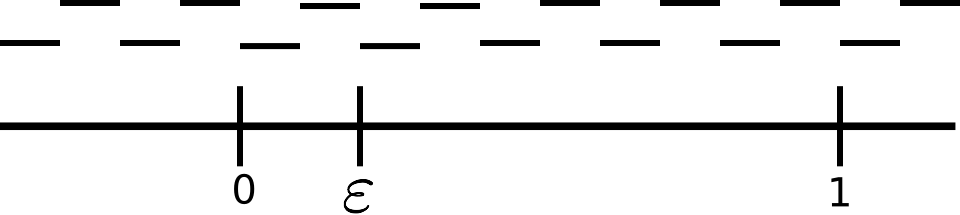
\includegraphics[width=0.3\textwidth]{Images/num4.png}
					\caption{Example of a $1$-periodic coefficient $A_1$ and it's scaling by $\varepsilon$}
					\label{fig4}
				\end{figure}
			\begin{assumption}
				Assume that $A\in L^\infty_{\text{per}}(0,1)$ is $1$-periodic and define the $\varepsilon$-periodic coefficients $A_\varepsilon$ (see also \cref{fig4}) by
				\[
					A_\varepsilon(x)\coloneqq A_1\left(\frac{x}{\varepsilon}\right).
				\]
			\end{assumption}
			\textbf{Question (more precisely):} Is there an effective (constant) coefficient $A_0>0$ such that the solution $u_\varepsilon$ of our model problem converge to $u_0$, the solution of the problem from \cref{c1se3su1}, uniformly w.r.t $f\in L^2(0,1)$.\newline\noindent
			If the answer is yes, then $A_0$ (resp. the problem) is called \textbf{homogenized/effective coefficient} (resp. solution, problem,...). There is the \underline{equally important} question of computability of $A_0$!\newline\newline\noindent

			In the simple $1$d model, we will be able to answer both questions in a stroke! \newline\noindent Assume for the time being that $A_0>0$ exists. (We restrict ourselves to the case $\varepsilon^{-1}\in\mathbb{N}$). We shall look at the $L^2$-error 
			\[
				u_\varepsilon-u_0 \in H^1_0(0,1)\subset L^2(0,1).
			\]
			There exists a unique $z\in H^1_0(0,1)$ such that
			\[
				\int_0^1  A_0z'w'\,dx = \int_0^1 (u_\varepsilon-u_0)w\,dx,\quad\forall w\in H^1_0(0,1).
			\]
			The choice $w = u_\varepsilon-u_0$ yields
			\[
				\|u_\varepsilon-u_0\|_{L^2(0,1)}^2 = \int_0^1 A^0 z'(u_\varepsilon-u_0)' \,dx
			\]
			(see the \textbf{Aubin-Nitsche duality trick})\newline\noindent
			The solutions $U_0$ and $u_\varepsilon$ are linked by the equality of the fluxes
			\[
				(A_0u_0')' = -f = (A_\varepsilon u_\varepsilon)'
			\]
			so they coincide up to a constant, i.e.
			\[
				A_0u_0' = A_\varepsilon u_\varepsilon'\quad\text{in }H^{-1}(0,1) = [H^1_0(0,1)]^*.
			\]
			Thus we have
			\[
				\int_0^1 (A_0u_0')w' \,dx= - \int_0^1 fw\,dx  = \int_0^1 (A_\varepsilon u_\varepsilon')w'\,dx,\quad\forall w\in H^1_0.
			\]
			This yields 
			\begin{IEEEeqnarray*}{rCl}
				\|u_\varepsilon - u_0\|_{L^2(0,1)}^2 &=& \int_0^1 z'(A_0-A_\varepsilon)u_\varepsilon' \,dx\\
				&=& \overbrace{\sum_{j=1}^{\varepsilon^{-1}}}^{\eqqcolon N} \int_{(j-1)\varepsilon}^{j\varepsilon} z'(A_0-A_\varepsilon)u_\varepsilon'\,dx\\
				&\overset{(*)}=& \sum_{j=1}^N \int_{(j-1)\varepsilon}^{j\varepsilon} \left( z'-\varepsilon^{-1}\int_{(j-1)\varepsilon}^{j\varepsilon} z'(s)\,dS \right)(A_0-A_\varepsilon)u_\varepsilon'\,dx \\&&+ \sum_{j=1}^N\left(\varepsilon^{-1} \int_{(j-1)\varepsilon}^{j\varepsilon} z'(s)\,dS \right)\int_{(j-1)\varepsilon}^{j\varepsilon} (A_0-A_\varepsilon)\left( u_\varepsilon' - \varepsilon^{-1}\int_{(j-1)\varepsilon}^{j\varepsilon}u_\varepsilon'(s)\,dS \right)\,dx \\ &&+ \sum_{j=1}^N \varepsilon^{-2} \int_{(j-1)\varepsilon}^{j\varepsilon} z'(s)\,dS\int_{(j-1)\varepsilon}^{j\varepsilon} u_\varepsilon'(s)\,dS\int_{(j-1)\varepsilon}^{j\varepsilon}(A_0-A_\varepsilon)\,dx
			\end{IEEEeqnarray*}
			Note that in $(*)$ we have added a zero, namely the mean value of $z'$. We have that $z$ is the solution of a Poisson problem with a constant RHS, so it is in $H^2$. Thus it's derivative is still in $H^1$. Unfortunately for $u_\varepsilon$ we just know that it is in $L^2$, so we have no regularity for $u_\varepsilon'$. Thus we make a further modification:
			\begin{IEEEeqnarray*}{rCl}
				\|u_\varepsilon - u_0\|_{L^2(0,1)}^2 &=& \int_0^1 z'(A_0-A_\varepsilon)u_\varepsilon' \,dx\\
				&=& \overbrace{\sum_{j=1}^{\varepsilon^{-1}}}^{\eqqcolon N} \int_{(j-1)\varepsilon}^{j\varepsilon} z'(A_0-A_\varepsilon)u_\varepsilon'\,dx\\
				&\overset{(*)}=& \sum_{j=1}^N \int_{(j-1)\varepsilon}^{j\varepsilon} \left( z'-\varepsilon^{-1}\int_{(j-1)\varepsilon}^{j\varepsilon} z'(s)\,dS \right)\frac{(A_0-A_\varepsilon)}{\color{red}{A_\varepsilon}}\color{red}{A_\varepsilon u_\varepsilon'}\,dx \\
				&&+ \sum_{j=1}^N\left(\varepsilon^{-1} \int_{(j-1)\varepsilon}^{j\varepsilon} z'(s)\,dS \right)\int_{(j-1)\varepsilon}^{j\varepsilon} \frac{(A_0-A_\varepsilon)}{\color{red}{A_\varepsilon}}\left( \color{red}{A_\varepsilon u_\varepsilon'}\color{black} - \varepsilon^{-1}\int_{(j-1)\varepsilon}^{j\varepsilon}\color{red}{A_\varepsilon u_\varepsilon'}\color{black}\,dS \right)\,dx \\ 
				&&+ \sum_{j=1}^N \varepsilon^{-2} \int_{(j-1)\varepsilon}^{j\varepsilon} z'(s)\,dS\int_{(j-1)\varepsilon}^{j\varepsilon} \color{red}{A_\varepsilon}\color{black}u_\varepsilon'(s)\,dS\int_{(j-1)\varepsilon}^{j\varepsilon}\frac{(A_0-A_\varepsilon)}{\color{red}{A_\varepsilon}}\color{black}\,dx.
			\end{IEEEeqnarray*}
			The third term on the right-hand side tends to $0$ (as $\varepsilon\to 0$) if and only if it is actually $0$, i.e.
			\[
				A_0 = \cancel{\varepsilon}\left( \varepsilon^{-1}\int_{(j-1)\varepsilon}^{j\varepsilon} A_\varepsilon^{-1}\,dx \right)^{-1}
			\]
			is chosen as the harmonic mean of $A_\varepsilon$. With this choice of $A_0$ and \emph{Cauchy-Schwarz} we get
			\begin{IEEEeqnarray*}{rCl}
				\|u_\varepsilon-u_0\|_{L^2(0,1)}^2 &\leq& \sum_{j=1}^N \left\| \frac{A_0-A_\varepsilon}{A_\varepsilon} \right\|_{L^\infty(0,1)}\\
				&& \cdot \bigg\{  \|z'-\overline{z'}\|_{L^2((j-1)\varepsilon,j\varepsilon)}\|A_\varepsilon u_\varepsilon'\|_{L^2((j-1)\varepsilon,j\varepsilon)} \\&&+ \|\overline{z'}\|_{L^2((j-1)\varepsilon,j\varepsilon)}\|A_\varepsilon u_\varepsilon'- \overline{A_\varepsilon u_\varepsilon'}\|_{L^2((j-1)\varepsilon,j\varepsilon)} \bigg\}\\
				&\leq& \frac{\varepsilon}{\pi}\left\|\frac{A_0-A_\varepsilon}{A_\varepsilon}\right\|_{L^\infty(0,1)}\sum_{j=1}^N\bigg( \|z''\|_{L^2((j-1)\varepsilon,j\varepsilon)}\|A_\varepsilon u_\varepsilon'\|_{L^2((j-1)\varepsilon,j\varepsilon)}\\&& + \|z'\|_{L^2((j-1)\varepsilon,j\varepsilon)}\|(A_\varepsilon u_\varepsilon')'\|_{L^2((j-1)\varepsilon,j\varepsilon)} \bigg).
			\end{IEEEeqnarray*}
			Define now constants $\alpha,\beta$ and assume that $\alpha\leq A_\varepsilon\leq \beta$. Then we have (continuing the previous estimate and using discrete Cauchy-Schwarz):
			\begin{IEEEeqnarray*}{rCl}
				&\leq& \frac{\varepsilon}{\pi}\left(\frac{\beta}{\alpha}+1\right) \left( \|z''\|_{L^2(0,1)} \|A_\varepsilon u_\varepsilon'\|_{L^2(0,1)} +  \|z'\|_{L^2(0,1)} \|(A_\varepsilon u_\varepsilon')'\|_{L^2(0,1)} \right)
			\end{IEEEeqnarray*}
			where $\alpha,\beta$ are chosen as
			\begin{IEEEeqnarray*}{rCl}
				\alpha&\coloneqq& \inf_{0\leq x\leq 1} A_1(x)\\
				\beta&\coloneqq&\sup_{0\leq x\leq 1}A_1(x).
			\end{IEEEeqnarray*}
			Continuing we get
			\begin{IEEEeqnarray*}{rCl}
				&\leq& \frac{\varepsilon}{\pi}\left(\frac{\beta}{\alpha}+1\right)\|u_\varepsilon-u_0\|_{L^2(0,1)}\sqrt{\frac{\beta}{\alpha}}\|f\|_{L^2(0,1)} + \frac{\|u_\varepsilon-u_0\|_{L^2(0,1)}}{\sqrt{A_0}}\|f\|_{L^2(0,1)}\\
				&\leq& \frac{\varepsilon}{\pi} \left(\frac{\beta}{\alpha}+1\right)\left(\sqrt{\frac{\beta}{\alpha}}+\frac{1}{A_0}\right)\|f\|_{L^2(0,1)}\|u_\varepsilon-u_0\|_{L^2(0,1)}.
			\end{IEEEeqnarray*}
			This shows that 
			\[
				\|u_\varepsilon-u_0\|_{L^2(0,1)} \leq C\varepsilon\|f\|_{L^2(0,1)}
			\]
			with constant
			\[
				C\coloneqq \frac{1}{\pi}\left(1+\frac{\beta}{\alpha}\right)\left(\frac{\sqrt{\beta}+1}{\sqrt{\alpha}}+1\right).
			\]
			Hence, for the choice 
			\[
				A_0 \coloneqq \left(\dashint_0^1 A_1^{-1}(x)\,dx\right)^{-1},
			\]
			we have $u_\varepsilon\overset{\varepsilon\to 0}\longrightarrow u_0$ strongly in $L^2(0,1)$.